% \documentclass{emulateapj}
\documentclass[letterpaper,12pt,preprint]{aastex}

\input{../paper-helpers/preamble.tex}

% packages
\usepackage{amssymb,amsmath,amsbsy}
\usepackage{booktabs}
\usepackage[caption=false]{subfig}
\usepackage{multirow}

\newcommand{\DM}{{\rm DM}}
\newcommand{\norm}{\mathcal{N}}

% TO DO
\usepackage{graphicx} 
\usepackage{color}
\newcommand{\todo}[1]{{\color{red} TODO: #1}}

\begin{document}

\title{Spending too much time at the Galactic bar: Chaotic evolution of the Ophiuchus stream}
\author{Adrian M. Price-Whelan\altaffilmark{\colum,\adrn},
            Branimir Sesar\altaffilmark{\mpia}, 
            Kathryn V. Johnston\altaffilmark{\colum},
            Hans-Walter Rix\altaffilmark{\mpia}
}

% Affiliations
\newcommand{\colum}{1}
\newcommand{\adrn}{2}
\newcommand{\mpia}{3}

\altaffiltext{\colum}{Department of Astronomy,
                      Columbia University,
                      550 W 120th St.,
                      New York, NY 10027, USA}
\altaffiltext{\adrn}{To whom correspondence should be addressed: adrn@astro.columbia.edu}
\altaffiltext{\mpia}{Max-Planck-Institut f\"ur Astronomie,
                     K\"onigstuhl 17, D-69117 Heidelberg, Germany}
                     
\begin{abstract}

% Context
The Ophiuchus stream was recently discovered as an over-density of main sequence stars in Pan-STARRS (PS1) photometry and was later detected in BHB stars using line-of-sight velocities: XX of the YY BHB stars around the sky position of the stream appear kinematically distinct from the background halo population.
A small number of stars (XX) near the ends of the stream have similarly distinct velocities but with much larger velocity and spatial dispersions compared to the short segment of the stream first identified in the PS1 data.
In recent work, we have shown that streams formed on chaotic orbits may display similar kinematic signatures---short segments of recently-disrupted stellar debris flanked by high-dispersion, low-density ``stream-fans'' at the ends of the stream.
The stream's proximity to the triaxial, time-dependent potential of the Galactic bar and the peculiar kinematics and morphology of the stream suggest that the stream may have formed on a chaotic orbit.
% Aims
Here we study whether the Galactic bar can lead to chaotic orbits near (in phase-space) to the Ophiuchus stream. 
% Methods
We construct a potential model for the Milky Way bar based on recent measurements of the density of XXX stars.
We then assess the level of chaos for orbits like that of the Ophiuchus stream and generate mock streams along these orbits that qualitatively reproduce the observed kinematics of the stream.
% Results
We find that the apparent shortness and nearby low-density, high-velocity-dispersion ...
% Conclusions
These results motivate efforts to obtain deep photometry of the region surrounding the Ophiuchus stream to detect the predicted low-surface-brightness fans of stellar debris.
The existence of or lack of stream fans may provide an interesting constraint on the triaxiality and pattern speed of the bar.

\end{abstract}

% \keywords{}

\section{Introduction}\label{sec:introduction}

The Ophiuchus stream \citep{bernard14, sesar15a} is a recently discovered stellar tidal stream that sits above the Galactic bulge at a Galactocentric radius and height $(R,z) \approx (1, 4.3)~{\rm kpc}$. All observational evidence suggests that the stream is a totally disrupted globular cluster: The stream stars have (1) a small positional dispersion orthogonal to the extended direction of the stream ($\approx$10 pc); (2) no detectable over-density along the stream that could be the progenitor system; (3) a small velocity dispersion $\approx$0.4 ${\rm km}~{\rm s}^{-1}$; and (4) an old stellar population ($\approx$12 Gyr) estimated from isochrone fitting \citep[][hereafter S15a]{sesar15a}. 

There are a number of peculiarities about the observed kinematics of probable member stars of the Ophiuchus stream. For example, the de-projected length of the visible part of the stream is short given the age of its stellar population ($\approx$1.5 kpc). S15a fit an orbit to the kinematics of the stream stars in a static, axisymmetric model for the gravitational field of the inner Galaxy and ran N-body simulations of globular clusters on this orbit. S15a find that---on this orbit---the portion of the stream visible as an over-density in main-sequence stars must have been formed in the last $\lesssim$400 Myr for the stream to remain as short as it is observed. This dynamical age is at odds with the old stellar population. Another puzzle is the existence of blue horizontal branch (BHB) stars close to the stream (within XX deg) with similar radial velocities, but with a large dispersion in both sky position and velocity \citep[][hereafter S15b]{sesar15b}. The stream has a very distinct and large line-of-sight velocity ($\approx$290 \kms) and is therefore easily detected above the background halo population. Four stars have been detected with line-of-sight velocities $>230~\kms$ that lie close to an extrapolation of the stream on the sky, but have a velocity dispersion $\approx$75 times larger than the measured internal velocity dispersion of the stream stars. These stars hint at the existence of associated low-density, high-dispersion features that were not modeled in S15a and are not predicted by the $N$-body simulations from this prior work.

The orbit fit and $N$-body simulations in S15a used a static, axisymmetric potential to represent the Milky Way potential, but it is now well-known that the Galactic bulge contains a triaxial, bar-like structure several kpc in size \citep[e.g.,][]{blitzXX, wegg13, MANY}. Given the proximity of the stream to the center of the Galaxy, the time-dependent, triaxial potential of the Galactic bar must be taken into account when modeling the orbit of the Ophiuchus stream. The presence of a bar-like perturbation to the potential will change the orbit of the stream progenitor and the orbit structure in the inner galaxy \citep{athanassoula, portail15b, zotos12}. Bar-like features can also introduce a significant number of chaotic orbits in their vicinity\citep{weinberg15}.

Recent work has shown that chaos can dramatically alter the density evolution of tidal streams. Along certain chaotic orbits, the stream stars will spread much faster in 3D position than from ordinary phase-mixing and, depending on the orbital phase at which the stream is observed, may develop large, low-density ``fans'' of stars at the ends of a stream \citep{apw15-chaos}. In this work, we study whether stream-fanning---chaotic or simply from density evolution in a triaxial, time-dependent potential---can explain the observed properties of the Ophiuchus stream. In particular, we consider a model successful if it qualitatively reproduces:
\begin{enumerate}
	\item the apparent shortness and fast density truncation of the stream;
	\item the increased positional dispersion of the four new candidate members from S15b;
	\item the much larger velocity dispersion of the S15b stars.
\end{enumerate}

In Section~\ref{sec:method} we describe the methods used in this work: in Section~\ref{sec:potential} we describe the models we use for the gravitational potential of the Galaxy, in Section~\ref{sec:mocks} we explain the simple method we use to generate mock streams, and in Section~\ref{sec:chaos-indicator} we briefly describe the methods we use for detecting and characterizing chaotic orbits. In Section~\ref{sec:results1} we discuss the differences in the orbit structure between a static, axisymmetric potential model and a model with a time-dependent bar potential, and in Section~\ref{sec:results2} we use mock streams to argue that [chaotic stream-fanning is a plausible explanation for the observational peculiarities of the Ophiuchus stream.] We conclude in Section~\ref{sec:conclusions}.

\section{Methods}\label{sec:method}

Our goal is to (1) assess whether the Galactic bar can produce chaotic orbits in the vicinity of the Ophiuchus stream and (2) determine if chaotic density evolution of tidal debris stripped from the progenitor of this stream can explain the apparent shortness of the stream and low-density, high-dispersion ends. In this section, we describe the potential models we use to represent the galaxy and describe the methods we use to detect and quantify the strength of chaos for orbits. We then describe the method we use for fitting orbits to the stream stars. Finally, we describe the method we use to generate mock stellar streams. 

\subsection{Potential models}\label{sec:potential}

To integrate orbits and to compute chaos indicators we must choose a gravitational potential model to represent the potential of the Milky Way. The key feature of the potential that we would like to capture is the time-dependence and triaxiality of the Galactic bar. Recent work has used stellar number counts of \todo{XX} stars in the Galactic bulge to constrain dynamical models of the bar \citep{portail15}. Measurements of the total mass of the bar feature from this study are largely consistent with past work \citep[e.g.,][]{XX}, however the measured pattern speed and present bar angle are significantly discrepant and this difference is not fully understood. We construct a parametrized potential model consisting of a triaxial, time-dependent (rotating) bulge component added to simple models for the disk and halo of the Milky Way. We describe below how we fix the parameters of the disk, halo, and bar or bulge component, but explore different choices for the time-dependence and orientation of the bar. We also define a static potential with a spherical bulge for comparison. These potential models are meant to be representative rather than definitive since the potential of the inner and outer Milky Way are not well known. 

\subsubsection{Barred potential}
We use a flattened Navarro-Frenk-White potential to represent the dark matter halo \citep[e.g.,][]{kuepper15} parametrized as
\begin{align}
	\Phi(r) &= -v_h^2\,\frac{\ln{(1 + r/r_s)}}{r/r_s}\label{eq:flatnfw}\\
	r^2 &= x^2 + y^2 + \frac{z^2}{q_z^2}
\end{align}
and a Miyamoto-Nagai potential for the disk \citep{miyamoto75}. For the bar component, we use a basis function expansion (BFE) of the potential and density of the bar with expansion coefficients derived for a triaxial, exponential bar density \citep[][hereafter W12]{wang12}. We use the pre-computed expansion coefficients used in W12, which were computed from a low-order expansion of the triaxial bar density used in \citet{dwek95}.\footnote{The coefficients presented in W12 are for just the cosine terms (the $A_{lm}$ in \citet{hernquist92} or the $S_{nlm}$ in \citet{lowing11}) because all sine terms have zero coefficients for a triaxial density function.} We have implemented the BFE computation of the potential, density, and gradient of the potential in \texttt{C} and \python\ and the code is publicly available on \github.\footnote{\url{https://github.com/adrn/biff}} 

The BFE representation fixes the axis ratios of the bar---that is, the the exponential scale lengths along the three axes of the bar were adopted from \cite{dwek95} when the expansion coefficients were calculated in W12); all other potential parameter values are given in Table~\ref{tbl:potential-params-barred}. The mass of the halo is fixed and the mass of the disk and bar are varied in order to qualitatively reproduce the flatness and amplitude of the circular velocity curve of the Milky Way \citep{bovy12}. Figure~\ref{fig:circ-vel-barred} shows the circular velocity along the line connecting the Sun to the Galactic center in this model (the Galactic $x$ axis). Figure~\ref{fig:surface-density-barred} shows contours of constant surface density for a face-on (left) and edge-on (right) view of this potential model with the bar angle set to $20^\circ$ \citep[compare to, e.g., Figure 3 in][]{portail15}. We consider a grid of nine parameter combinations of bar angle and pattern speed. These model names and parameter values are given in Table~\ref{tbl:bar-specific}.

\begin{table*}[ht]
\begin{center}
	\begin{tabular}{ c | c | c }
	         \toprule
	         Component & Parameter & Value \\\toprule
		Disk & $M_{\rm disk}$ & $5 \times 10^{10}~\msun$ \\
		& $a$ & 3~{\rm kpc}\\
		& $b$ & 0.28~{\rm kpc} \\\midrule
	         Halo & $v_c$ & 185.8~\kms\\
		& $r_s$ & 30~kpc \\
		& $q_z$ & 0.9 \\\midrule
		Bar & $M_{\rm bar}$ & $1.8 \times 10^{10}~\msun$ \\
		\bottomrule
		\end{tabular}
	\caption{The disk potential scale lengths ($a$, $b$) were adopted following \citep{bovy15-galpy} to match the exponential scale length of the disk \citep{bovyrix13} and local dark-matter density \citep[e.g.,][]{bovytremaine12}. Halo flattening is taken from recent work that suggests the inner Milky Way halo is slightly oblate \citep{koposov10, kuepper15}. The halo mass scale is set by specifying the circular velocity at the scale radius, $v_c$, and the scale velocity in Equation~\ref{eq:flatnfw} is given by $v_h^2 = v_c^2 / (\ln2 - 1/2)$. The bar mass is taken from recent 3D density modeling of red clump stars in the Galactic bulge \citep{portail15}. The other bar parameters are listed in Table~\ref{tbl:bar-specific} next to the corresponding model name. \label{tbl:potential-params-barred}}
\end{center}
\end{table*}

\begin{table*}[ht]
\begin{center}
	\begin{tabular}{ c | c | c }
	         \toprule
	         Name & $\alpha$ [deg] & $\Omega_p$ [${\rm km}~{\rm s}^{-1}~{\rm kpc}^{-1}$] \\\toprule
		bar1 & 20 & 40\\
		bar2 & 20 & 50\\
		bar3 & 20 & 60\\
		bar4 & 25 & 40\\
		bar5 & 25 & 50\\
		bar6 & 25 & 60\\
		bar7 & 30 & 40\\
		bar8 & 30 & 50\\
		bar9 & 30 & 60\\
		\bottomrule
		\end{tabular}
	\caption{Present-day bar angle ($\alpha$) and pattern speed ($\Omega_p$) for the nine parameter pairs considered in this work. These values span the range of recent measurements from a variety of techniques \citep{dwek95,wang12,wang13, MOREMOREMORE}. \label{tbl:bar-specific}}
\end{center}
\end{table*}

\subsubsection{Static potential}

For comparison, we also define a time-independent potential model with a purely spherical bulge. In this model, we set the bar mass to 0 and instead add a spheroidal component represented with a Hernquist potential \citep{hernquist90}. Parameters for this potential model are given in Table~\ref{tbl:potential-params-static}. Figure~\ref{fig:circ-vel-barred} shows the circular velocity along the line connecting the Sun to the Galactic center in this model (the Galactic $x$ axis). Figure~\ref{fig:surface-density-static} shows contours of constant surface density for a face-on (left) and edge-on (right) view of this potential model.

\begin{table*}[ht]
\begin{center}
	\begin{tabular}{ c | c | c }
	         \toprule
	         Component & Parameter & Value \\\toprule
		Disk & $M_{\rm disk}$ & $6.5 \times 10^{10}~\msun$ \\
		& $a$ & 3~{\rm kpc}\\
		& $b$ & 0.28~{\rm kpc} \\\midrule
	         Halo & $v_c$ & 185.8~\kms\\
		& $r_s$ & 30~kpc \\
		& $q_z$ & 0.9 \\\midrule
		Spheroid & $M_{\rm sph}$ & $10^{10}~\msun$ \\
		& $c$ & 0.2 \\
		\bottomrule
		\end{tabular}
	\caption{Same as Table~\ref{tbl:potential-params-barred}, except: the disk mass is increased to account for removing the bar component, a spheroidal bulge component is added. \label{tbl:potential-params-static}}
\end{center}
\end{table*}

\subsection{Fitting orbits to the Ophiuchus stream}\label{sec:orbitfit}

In each of the potentials described above, we fit orbits to the measured kinematics of BHB stars that are high-likelihood members of the Ophiuchus stream \citep{sesar15a, sesar15b}. Our goal is to infer the posterior probability distributions over orbital initial conditions, $\bs{w}_0=(l, b, \DM, \mu_l, \mu_b, v_r)_0$, given a potential, $\Phi$, and kinematic data for each $i$ stream star, $\bs{x}_i=(l, b, \DM, \mu_l, \mu_b, v_r)_i$. In this notation, $(l, b)$ are Galactic coordinates, $\DM$ is the distance modulus, $(\mu_l, \mu_b)$ are proper motions in the Galactic frame, and $v_r$ is the radial velocity. We assume that the sky coordinates for each star are known perfectly well (have zero uncertainty) and transform the data to a rotated, heliocentric coordinate system that is aligned with the stream and centered on the median sky position of the BHB stars in the densest part of the stream \cite[all BHB stars except the `fanned' stars: cand15, cand26, cand49, cand54 from][]{sesar15b}. We represent the longitude and latitude in these coordinates as $(\phi_1, \phi_2)$ and the rotation matrix to transform from Galactic to these coordinates is given in Appendix~\ref{sec:rotationmatrix}. We treat the stream longitude, $\phi_1$, as the perfectly-known, independent variable so that all other coordinates can be expressed as functions of this longitude (e.g., $\phi_2(\phi_1)$, ${\rm DM}(\phi_1)$, etc.). This methodology is similar to that used in \cite{koposov10} and \cite{sesar15a}.

\subsubsection{Likelihood}

We include three nuisance parameters in our likelihood to account for the internal dispersion of the stream: in observed coordinates, these are the on-sky positional dispersion, $s_{\phi_2}$, a distance (modulus) dispersion, $s_{\DM}$, and a radial velocity dispersion, $s_{v_r}$ (the proper motion uncertainties are sufficiently large that we can't resolve the velocity dispersion in these coordinates).\footnote{We assume that the dispersion in these coordinates is constant over the observed (short) section of the stream. This may be a bad assumption.} We add two additional nuisance parameters for controlling the amount of time to integrate forwards, $t_f$, and backwards, $t_b$, from the given initial conditions, which ultimately controls the length of the section of orbit that is compared to the stream star data. For brevity in the equations below, we define $\bs{s} = (s_{\phi_2}, s_{\DM}, s_{v_r})$ and $\bs{\theta} = (\bs{w}_0, \Phi, t_b, t_f)$.

For a given set of initial conditions ($\bs{w}_0$), we compute a model orbit as follows: (1) transform the initial conditions to Galactocentric coordinates, where we take the position and velocity of the Sun to be 
\begin{align}
	(x,y,z)_\odot &= (-8,0,0)~{\rm kpc}\\
	(v_x,v_y,v_z)_\odot &= (-11.1, 220+24, 7.25)~{\rm km}~{\rm s}^{-1}
\end{align}
\citep{8kpref??, schonrich10, bovy12}, (2) integrate the orbit forward and backward by $t_f$ and $t_b$, respectively, in the potential $\Phi$, (3) transform all orbit points (time-steps) back to observed coordinates, and (4) define interpolating functions for each coordinate as a function of stream longitude, $\phi_1$, using cubic splines---e.g., functions $\widetilde{\phi}_{2}(\phi_1)$, $\widetilde{\DM}(\phi_1)$, $\widetilde{\mu_l}(\phi_1)$, $\widetilde{\mu_b}(\phi_1)$, $\widetilde{v_r}(\phi_1)$. These functions let us compute the predicted values of each of these coordinates at the longitudes of each observed star, $\phi_{1,i}$.

We assume that each observed kinematic component is independent so that the likelihood of the data for a given star, $\bs{x}_i$, with uncertainties, $\bs{\sigma}_i$, is given by the product over the likelihoods for each dimension of the data:
\begin{multline}
	p(\bs{x}_i \given \bs{\sigma}_i, \bs{s}, \bs{\theta}) = p(\phi_{2,i} \given \phi_{1,i}, s_{\phi_2},\bs{\theta}) \, p(\DM_i \given \phi_{1,i}, \sigma_{\DM,i}, s_\DM, \bs{\theta})\\ 
	\times p(\mu_{l,i} \given \phi_{1,i}, \sigma_{\mu_{l},i}, \bs{\theta}) \, p(\mu_{b,i} \given \phi_{1,i}, \sigma_{\mu_{b},i}, \bs{\theta}) \, p(v_{r,i} \given \phi_{1,i}, \sigma_{v_r,i}, s_{v_r}, \bs{\theta}).
\end{multline}
The uncertainties in these observed coordinate components are assumed to be normally distributed away from the model values: using the notation
\begin{align}
	\norm(x \given \mu, \sigma^2) &= \frac{1}{\sqrt{2\pi \sigma^2}} \, \exp\left(-\frac{(x-\mu)^2}{2\sigma^2}\right)
\end{align}
the likelihoods are
\begin{align}	
	p(\phi_{2,i} \given \phi_{1,i}, s_{\phi_2},\bs{\theta}) &= \norm(\phi_{2,i} \given \widetilde{\phi}_{2}(\phi_{1,i}), s^2_{\phi_2})\\
	p(\DM_i \given \phi_{1,i}, \sigma_{\DM,i}, s_\DM, \bs{\theta}) &= \norm(\DM_i \given \widetilde{\DM}(\phi_{1,i}), s^2_{\DM} + \sigma^2_{\DM,i})\\
	p(\mu_{l,i} \given \phi_{1,i}, \sigma_{\mu_{l},i}, \bs{\theta}) &= \norm(\mu_{l,i} \given \widetilde{\mu_{l}}(\phi_{1,i}), \sigma^2_{\mu_{l,i}})\\
	p(\mu_{b,i} \given \phi_{1,i}, \sigma_{\mu_{b},i}, \bs{\theta}) &= \norm(\mu_{b,i} \given \widetilde{\mu_{b}}(\phi_{1,i}), \sigma^2_{\mu_{b,i}})\\
	p(v_{r,i} \given \phi_{1,i}, \sigma_{v_r,i}, s_{v_r}, \bs{\theta}) &= \norm(v_{r,i} \given \widetilde{v_r}(\phi_{1,i}), s^2_{v_r} + \sigma^2_{v_r,i}).
\end{align}
We assume the data from each star is independent and identically distributed (i.i.d.) so that the full likelihood is the product over the likelihoods for each star:
\begin{equation}
	 p(\{\bs{x}_i\} \given \{\bs{\sigma}_i\}, \bs{s}, \bs{\theta}) = \prod_i p(\bs{x}_i \given \bs{\sigma}_i, \bs{s}, \bs{\theta}).\label{eq:likelihood}
\end{equation}

\subsubsection{Priors}

For the intrinsic dispersion parameters, we use logarithmic (scale-invariant) priors such that $p(s) \propto s^{-1}$. For the integration time parameters, we use uniform priors, $\mathcal{U}(a,b)$ (over the range $a$--$b$),
\begin{align}
	p(t_f) &= \mathcal{U}(1,100)~{\rm Myr}\label{eq:prior1}\\
	p(t_b) &= \mathcal{U}(-100,-1)~{\rm Myr}.
\end{align}
Note that present-day is $t=0$. For computational efficiency, we place strong priors on the minimum and maximum longitudes of the model points, $(\phi_{1,{\rm min}},\phi_{1,{\rm max}})$ so that the model orbit does not integrate for longer than necessary. In particular, we set
\begin{align}
	p(\phi_{1,{\rm min}} \given \bs{\theta}) &= \norm(\phi_{1,{\rm min}} \given \min(\phi_{1,i}), s^2_{\phi_2})\\
	p(\phi_{1,{\rm max}} \given \bs{\theta}) &= \norm(\phi_{1,{\rm max}} \given \max(\phi_{1,i}), s^2_{\phi_2}).
\end{align}
For the orbital initial condition components, we use uniform priors in each cartesian position component over the range $(-200,200)~{\rm kpc}$. For velocity, we use a Gaussian prior on the magnitude of the total velocity, $v$, with a dispersion of $150~\kms$,
\begin{equation}
	\norm(v \given 0, (150~\kms)^2) \label{eq:prior2}
\end{equation}
We keep the potential, $\Phi$, fixed. In total, this model has 10 parameters (5 phase-space coordinates, 5 nuisance parameters).

\subsubsection{Sampling from the posterior distributions}

The full expression for the posterior probability, $p(\bs{s}, \bs{w}_0, t_b, t_f \given \{\bs{x}_i\}, \{\bs{\sigma}_i\}, \Phi)$, is the joint likelihood (Equation~\ref{eq:likelihood}) multiplied by all priors described above (Equations~\ref{eq:prior1}--\ref{eq:prior2}). We use an ensemble Markov Chain Monte Carlo (MCMC) algorithm \citep{goodman10} implemented in \python\ (\package{emcee}) to draw samples from this posterior distribution \citep{foremanmackey13}. The algorithm uses an ensemble of individual ``walkers'' to adapt to the geometry of the parameter-space being explored. In all cases, we use 80 walkers.

To initialize these walkers, we first run an optimization routine to maximize the likelihood. In detail, we use the Powell algorithm implemented in \package{Scipy} \citep{powell64, scipy} to minimize the negative, log-likelihood. To generate initial conditions for the walkers, we sample from Gaussian distributions centered on the maximum likelihood values. For the coordinates, we set the dispersions of these Gaussians to 1/1000 of the median uncertainties of the stars. For the nuisance parameters, we set the dispersions to 1/1000 of their maximum likelihood values. 

For each potential, we run the MCMC walkers for a burn-in period of 128 steps and then re-initialize the walkers from their positions at the end of this run. This erases any relics of the initialization procedure outlined above. After burn-in, we run the walkers for an additional 256 steps.
%
%\subsection{Detecting and characterizing chaos with frequency diffusion}\label{sec:chaos-indicator}
%
%Regular orbits are quasi-periodic: any phase-space component of the orbit can be decomposed in terms of a Fourier series, e.g.,
%\begin{equation}
%	x(t) = \sum^\infty_k \, a_{x,k}\, e^{i\, \omega_k \, t}.
%\end{equation}
%The amplitudes, $\bs{a}_k$ are constants which determine the strength of each mode, and the frequencies in each Fourier mode, $\omega_k$, are linear, integer combinations of the fundamental frequencies of the orbit, $\bs{\Omega}$---that is,
%\begin{equation}
%	\omega_k = \bs{n}_k \cdot \bs{\Omega}
%\end{equation}
%where $\bs{n}_k$ is a integer vector with dimensionality equal to the number of degrees of freedom of the gravitational potential \citep[e.g.,][]{binney82, binneytremaine}. The fundamental frequencies of a regular orbit are directly related to the orbital actions, a set of integrals of motion intricately related to the [...] of Hamiltonian and nonlinear dynamics \citep[e.g.,][]{??}. The fundamental frequencies can be approximated for numerically-integrated orbital time series by measuring the positions and amplitudes of spectral lines in the Fourier transform of the orbital components. A very accurate procedure for numerically computing the frequencies was developed by \citet{laskar93} and has been re-implemented in \python\ and released as open-source software \citep[\superfreq;][]{superfreq}. 
%
%Chaotic orbits have no actions and therefore no fundamental frequencies. The frequencies and actions drift erratically in time with rates that depend on the structure of resonances surrounding such orbits. The evolution of the frequencies changes the configuration-space appearance of finite sub-sections of chaotic orbits and greatly enhances the density evolution of ensembles of nearby chaotic orbits; this has a dramatic effect on the morphological evolution of tidal streams \citep[e.g.,][]{apw15-chaos}. Numerically-integrated trajectories can be identified as chaotic orbits by the detection of frequency diffusion \citep[e.g.,][]{laskar96, valluri98}. 
%
%The accuracy of the frequency-finding method (\superfreq) allows for detecting very small changes in the frequencies of even mildly chaotic orbits. Measuring the rate of frequency diffusion is therefore a powerful tool for detecting and characterizing dynamical chaos \citep[e.g.,][]{many}. From measuring the frequencies in many consecutive, overlapping time-windows along a numerically integrated orbit, we define the frequency diffusion rate, $DERP$, as
%\begin{equation}
%	yo
%\end{equation}
%where the index $k$ refers to the window number and $\tau$ is the shift in time between two consecutive windows. We note that this definition differs from previous, coarse approximations of the diffusion rate that simply differenced the frequencies computed in two consecutive time windows. We use this frequency diffusion rate to identify chaotic orbits integrated in the potential models described above.

\subsection{Generating mock streams}\label{sec:mocks}

To generate mock stellar streams, we use the method presented in \citep{fardal14}: star particles are `released' from a progenitor system near the Lagrange points with some dispersion in position and velocity set by the mass and orbit of the progenitor (this is similar to the \streakline\ method of \citet{kuepper12} but with finite dispersions). To generate progenitor orbits, we draw samples from the posterior probability distributions over orbital parameters from fitting orbits to the stream star members (Section~\ref{sec:orbit-fit}). For a given progenitor orbit---the 6D position of the orbit today---we integrate the orbit backwards in time for a given integration period. From the endpoint of the backwards-integration (e.g., the past position), we begin integrating the orbit forward in time, but now at each time-step a star particle is released near each of the Lagrange points of the progenitor. The position of the Lagrange points and the scale of the dispersion in position and velocity are set by the progenitor mass, $m$. The star particles are drawn from Gaussians centered on the Lagrange points (in position) and the progenitor (in velocity) and the full parametrization of the release distribution is given in \cite{fardal14}. This method has been shown to reproduce the morphologies of $N$-body simulations of stellar streams, but requires far less computing time because it relies only on integrating test-particle orbits.

\section{Results I: Orbit fits}\label{sec:results1}

Figures~\ref{fig:orbitfits1}--\ref{fig:orbitfits2} summarize our results from fitting orbits to the BHB stream stars. Shown in each panel are the Ophiuchus stream star members (black points) and samples from the  posterior probability over orbital parameters (blue lines). The end-to-end integration time of the orbit over the observed extent of the stream is only $\approx$6 Myr, so the derived orbits are extremely similar in all potentials (the time-dependence of the bar potential is not significant over such short timescales). The orbital periods are typically $\approx$150--250 Myr.

Though the orbital parameter values in observed coordinates are very similar between each potential model, the resulting orbits are quite different. Figure~\ref{fig:orbits-yz} shows projections of the ``mean'' orbits from each potential model; for each posterior distribution from orbit fitting, we take the mean values of the orbital parameters and convert to Galactocentric coordinates (e.g., Table~\ref{tbl:param-means}). For each orbit, we compute the maximum Lyapunov exponent (MLE, $\lambda$) to assess whether the orbit is chaotic.  Though not predictive for the timescale over which chaos is important for tidal debris, the MLE is still an appropriate indicator of chaos \citep{apw15-chaos}. Figure~\ref{fig:lyapunov} shows numerical estimates of the Lyapunov time ($t_\lambda = 1/\lambda$) for the mean orbits in each potential model: in the static potential the orbit appears regular (black, diagonal line), but in all barred potentials the MLE estimates converge to finite values in the range $\approx$2--8 orbital periods. \todo{Should I compute Lyapunov exponents for samples from the posterior, not just the mean orbit?}

The mean orbits in the barred potentials are all strongly chaotic. We have tried computing the frequency diffusion rate for these orbits but have found that, over two consecutive integration windows, the frequency recovery fails because the frequency spectrum changes dramatically over timescales of $\approx$10--20 orbital periods.

\begin{table*}[ht]
\footnotesize
\begin{center}
	\begin{tabular}{cccccc}
	\toprule
%	name & $\phi_2$ [deg] & $d$ [kpc] & $\mu_l$ [mas yr$^{-1}$] & $\mu_b$ [mas yr$^{-1}$] & $v_r$ [km s$^{-1}$] & $s_{\phi_2}$ [deg] & $s_{d}$ [kpc] & $s_{v_r}$ [km s$^{-1}$]\\\midrule
%static & $-0.03\pm0.05$ & $8.35\pm0.05$ & $-7.2\pm0.1$ & $0.9\pm0.1$ & $289.1\pm0.9$ & $0.20\pm0.04$ & $0.31\pm0.10$ & $2.9\pm0.8$\\
%bar1--9 & $-0.03\pm0.05$ & $8.40\pm0.05$ & $-7.2\pm0.1$ & $0.9\pm0.1$ & $289.0\pm1.0$ & $0.21\pm0.05$ & $0.31\pm0.14$ & $3.2\pm0.9$\\
	name & $\phi_2$ [deg] & $d$ [kpc] & $\mu_l$ [mas yr$^{-1}$] & $\mu_b$ [mas yr$^{-1}$] & $v_r$ [km s$^{-1}$]\\\midrule
	static & $-0.03\pm0.05$ & $8.35\pm0.05$ & $-7.2\pm0.1$ & $0.9\pm0.1$ & $289.1\pm0.9$\\
	bar1--9 & $-0.03\pm0.05$ & $8.40\pm0.05$ & $-7.2\pm0.1$ & $0.9\pm0.1$ & $289.0\pm1.0$\\
	\bottomrule
	\end{tabular}
	
	\begin{tabular}{ccc}
	\toprule
%	name & $\phi_2$ [deg] & $d$ [kpc] & $\mu_l$ [mas yr$^{-1}$] & $\mu_b$ [mas yr$^{-1}$] & $v_r$ [km s$^{-1}$] & $s_{\phi_2}$ [deg] & $s_{d}$ [kpc] & $s_{v_r}$ [km s$^{-1}$]\\\midrule
%static & $-0.03\pm0.05$ & $8.35\pm0.05$ & $-7.2\pm0.1$ & $0.9\pm0.1$ & $289.1\pm0.9$ & $0.20\pm0.04$ & $0.31\pm0.10$ & $2.9\pm0.8$\\
%bar1--9 & $-0.03\pm0.05$ & $8.40\pm0.05$ & $-7.2\pm0.1$ & $0.9\pm0.1$ & $289.0\pm1.0$ & $0.21\pm0.05$ & $0.31\pm0.14$ & $3.2\pm0.9$\\
	$s_{\phi_2}$ [deg] & $s_{d}$ [kpc] & $s_{v_r}$ [km s$^{-1}$]\\\midrule
	$0.20\pm0.04$ & $0.31\pm0.10$ & $2.9\pm0.8$\\
	$0.21\pm0.05$ & $0.31\pm0.14$ & $3.2\pm0.9$\\
	\bottomrule
	\end{tabular}
	\caption{Estimated mean and standard deviation of samples from the marginal posterior distributions over each parameter in our orbit fit model. For the barred potentials, all mean values are the same because the time-dependence of the bar doesn't impact the orbit fit over the short length of the stream. We have made samples from the full posterior distribution available with this article and provide code to transform to and from stream coordinates (see http://adrian.pw/ophiuchus/coordinates for more information).\label{tbl:param-means} }
\end{center}
\end{table*}


\section{Results 2: Stream models for the Ophiuchus stream}

\section{Discussion}\label{sec:discussion}

The model streams presented here do not reproduce all observed features of the Ophiuchus stream. Instead, these results illustrate that chaotic evolution of tidal debris can plausibly explain the peculiar features of the stream. If the cluster progenitor was on a regular orbit, it would have to have disrupted entirely within the last $\approx$300 Myr (Figure~\ref{TODO}) in order to explain the shortness and density profile. In addition, the four most recently identified BHB stars with similar distances and line-of-sight velocities would have to be (highly unlikely) chance alignments of halo stars. If instead the progenitor were on a chaotic orbit (because of the influence of the Galactic bar), (1) stars stripped early will have ``fanned'' out and would thus be harder to observe and (2) the nearby, high-velocity-dispersion BHB stars can be naturally explained by this chaotic stream-fanning. We consider the second scenario to be more plausible: our understanding of the formation and evolution of the Ophiuchus stream is that the progenitor object has been orbiting and steadily losing stars over the last several Gigayears, but only the stars stripped from the most recent few pericentric passages remain coherent enough to be detected as a stream-like over-density in the PS1 data.

[bar not well understood but maybe this stream can help distintuish models with more data -- cite discrepancy in measruements (antoja14, wang12, wang13)]

[Gaia, Don't do distance cut that Brani did, chemistry]

[explored in future work: what are implications of the existence of this structure for total population]

What is a successful model?
- Sharp density drop
	- BHB density falls off sooner? Is that just small-number statistics?
	- Density profile along the stream / how sharp is the drop?
	- Density contrast for BHB stars?
- Increased positional dispersion
	- The 4 new stars
- Velocity dispersion of the 4 new stars
	- velocity dispersion ~ 40 times internal velocity dispersion of stream stars
- What can we say about the connection between chaotic timescale and the length of the stream? Is it the onset time for chaos, or are all orbits strongly chaotic?
	- for a given orbit and model, paint the particles to say what the mass loss rate would have to be to match the obs.
- "It's stupid to make it more complicated" -- Kathryn Johnston
- from painting particles, Length of stream --> dispersion

\section{Conclusions}\label{sec:conclusions}

We have found that, with a qualitative but observationally-motivated potential model for the Galactic bar, the orbits of the Ophiuchus stream stars are likely sensitive to the time-dependence and shape of the bar potential. For modeling the stream itself, it is therefore crucial to include this component of the Galactic potential. By fitting orbits to kinematic data for members of the stream in Milky Way-like potential models, we have found that orbits in the vicinity of the Ophiuchus stream are strongly chaotic for a range of bar parameters (pattern speeds and present-day angles). Using mock stellar stream models generated assuming a globular cluster-mass progenitor object, we have shown that the apparent shortness of the stream and the existence of nearby stars with very high velocity dispersion are plausibly explained by chaotic density evolution of the stars stripped from the progenitor object. 

This is the first time chaos has been used to explain the morphology of a stellar stream and the first observational evidence for the importance of chaos in the Galactic halo. It also highlights the importance of including the Galactic bar in dynamical modeling of the Milky Way's inner halo and has important implications for future modeling of streams near in this region. With more Ophiuchus stream members, density and velocity information over a larger region near the stream, and better models for the internal structure of the Galactic bar, careful modeling of this stream could lead to tight constraints on the time-dependent properties of the bar.

\acknowledgements
APW is supported by a National Science Foundation Graduate Research Fellowship under Grant No.\ 11-44155.
APW acknowledges the staff at the MPIA for...
The authors wish to acknowledge Victor Debattista, ...
This research made use of Astropy, a community-developed core Python package for Astronomy \citep{astropy13}.
This work additionally relied on Columbia University's \emph{Yeti} compute cluster, and we acknowledge the Columbia HPC support staff for assistance. \\

\bibliographystyle{apj}
\bibliography{refs}

\appendix
\section{Transformation from Galactic to Ophiuchus stream coordinates} \label{sec:rotationmatrix}
The transformation matrix is approximately represented as
\begin{equation*}
\left( \begin{array}{c}
x \\
y \\
z \end{array} \right)_{\rm Oph} \approx
\left( \begin{array}{ccc}
0.84922096554 & 0.07001279040 & 0.52337554476\\
-0.27043653641 & -0.79364259852 &  0.54497294023\\
0.45352820359 & -0.60434231606 & -0.65504391727
\end{array} \right) \,
\left( \begin{array}{c}
x \\
y \\
z \end{array} \right)_{\rm Gal}
\end{equation*}
but the precise transformation and coordinate frame is implemented in \python\ using the \package{Astropy} coordinates package.\footnote{See \url{http://adrian.pw/ophiuchus/coordinates} for more information}  This code is hosted on \project{GitHub}.\footnote{\url{https://github.com/adrn/ophiuchus}} 

% ---------------------------------------------------------------------------------
\clearpage
\begin{figure}[p]
\begin{center}
\includegraphics[width=\textwidth]{figures/barred-circ-vel}
\caption{Circular velocity curve along the Sun-Galactic center line for the barred MW potential model. Solid black line shows total (sum of all components), lines below show a decomposition by potential component. Vertical grey bar shows approximate position of the Sun, horizontal grey bar shows roughly the range in measured circular velocity of the Sun.}
\label{fig:circ-vel-barred}
\end{center}
\end{figure}

% ---------------------------------------------------------------------------------
\clearpage
\begin{figure}[p]
\begin{center}
\includegraphics[width=\textwidth]{figures/barred-surface-density-contour}
\caption{Contours of constant surface density for two projections of the barred MW potential model. For both face-on view (left panel) and edge-on view (right panel), four contours are drawn per decade in surface density between $10^7$ and $10^{12}~\msun~{\rm kpc}^{-3}$. Note the perturbation from the bar potential within Galactocentric radius $r \lesssim 4~{\rm kpc}$. The Sun's position is indicated by the `$\odot$' symbol.}
\label{fig:surface-density-barred}
\end{center}
\end{figure}

% ---------------------------------------------------------------------------------
\clearpage
\begin{figure}[p]
\begin{center}
\includegraphics[width=\textwidth]{figures/static-circ-vel}
\caption{Same as Figure~\ref{fig:circ-vel-barred} for the static, axisymmetric MW potential model. }
\label{fig:circ-vel-static}
\end{center}
\end{figure}

% ---------------------------------------------------------------------------------
\clearpage
\begin{figure}[p]
\begin{center}
\includegraphics[width=\textwidth]{figures/static-surface-density-contour}
\caption{Same as Figure~\ref{fig:surface-density-barred} for the static, axisymmetric MW potential model. }
\label{fig:surface-density-static}
\end{center}
\end{figure}

% ---------------------------------------------------------------------------------
\clearpage
\begin{figure}[p]
\begin{center}
\includegraphics[width=\textwidth]{figures/orbitfits-0}
\caption{ Results from fitting orbits to BHB stars associated with the Ophiuchus stream in each potential model (see also Figure~\ref{fig:orbitfits2}). Data are shown as black points with grey error bars. Error bars may sometimes be smaller than the point size. Lines (blue) show sections of orbits integrated forward and backwards from initial conditions drawn from the posterior samples generated by MCMC (See Section~\ref{sec:orbitfit}). Note that the four higher dispersion stars (the four stars with highest longitude) were not used when computing the likelihood and are only shown for completeness. }
\label{fig:orbitfits1}
\end{center}
\end{figure}

\clearpage
\begin{figure}[p]
\begin{center}
\includegraphics[width=\textwidth]{figures/orbitfits-1}
\caption{Same as Figure~\ref{fig:orbitfits2} for the five other potential models.}
\label{fig:orbitfits2}
\end{center}
\end{figure}

% ---------------------------------------------------------------------------------
\clearpage
\begin{figure}[p]
\begin{center}
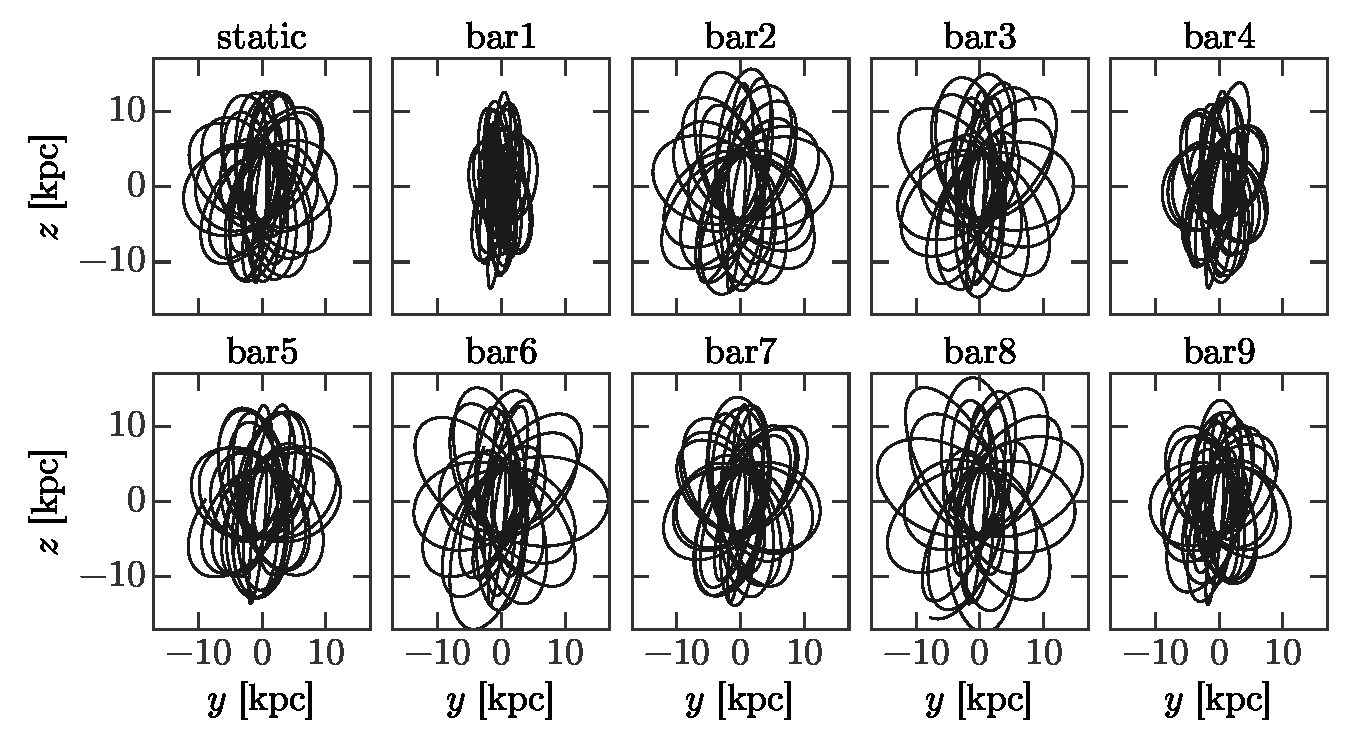
\includegraphics[width=\textwidth]{figures/orbit-yz}
\caption{  TODO }
\label{fig:orbits-yz}
\end{center}
\end{figure}

% ---------------------------------------------------------------------------------
\clearpage
\begin{figure}[p]
\begin{center}
\includegraphics[width=\textwidth]{figures/lyapunov}
\caption{ Estimates of the Lyapunov time, $t_\lambda=1/\lambda$, for the mean orbits in each potential model (Section~\ref{sec:results1}). All time units are given in units of orbital periods. The orbits are integrated from the mean values of orbital parameters from orbit fitting (Section~\ref{sec:orbitfit}). In the static, axisymmetric potential model, an orbit fit to the Ophiuchus stream is regular. In all barred potential models (bar1--9), the mean orbit is chaotic with a Lyapunov time that is less than 10 orbital periods. }
\label{fig:lyapunov}
\end{center}
\end{figure}


\end{document}